\subsection{Mechanism experiment: complete specification}
\label{sec:mechanisms-details}

The experiment uses an initial anchor, labeled zero, and 32 candidates
labeled $1,\ldots,32$.  Candidate batches are $1{:}4$, $5{:}8$,
$9{:}16$, $17{:}24$, and $25{:}32$, with arrival times given in the main
text.  The following definitions fix each mean vector before any reward
is simulated:
\begin{enumerate}
\item Near ties: the anchor has mean $0.52$; candidates have mean $0.50$,
except labels $4,8,16,24,32$, which have mean $0.515$.
\item Poor candidates: the anchor has mean $0.70$; candidate $i$ has mean
$0.10+0.05(i\bmod 4)$.
\item New record: the anchor has mean $0.45$; candidates have mean $0.35$,
except label $17$, which arrives at $\lfloor T/2\rfloor+1$ with mean $0.80$.
\item Mixed late batch: the anchor has mean $0.55$ and the first 24
candidates have mean $0.40$.  The last batch has means
$(0.15,0.35,0.52,0.58,0.62,0.72,0.48,0.20)$.
\item Near upper bound: the anchor has mean exactly one; candidates have
mean $0.94$, except labels $4,8,16,24,32$, which have mean $0.985$.
\end{enumerate}
In the reverse-order version, the reward distributions remain attached
to the same physical arms; only their positions within each candidate
batch change.  All index rules choose the first label among maximizers.
For the confidence-index rules, unobserved arms have infinite index,
except for clipped MC-MOSS, for which the index is one.
Thompson sampling instead draws independently from
$\operatorname{Beta}(1+S_i,1+N_i-S_i)$ for every present arm at each
decision.  An arriving arm begins with $N_i=S_i=0$, and none of these
baselines discards observations.  KL-UCB uses
\[
 U_i(t)=\sup\{q\in[\widehat\mu_i,1]:
 N_i\operatorname{kl}(\widehat\mu_i,q)\leq\log t\}.
\]
The scalar root is computed by 32 bisections, with an index error below
$2^{-32}$.  A monotonicity check skips a root only when its exact index
cannot exceed the current maximizer.  Neither the horizon, the means,
nor unrevealed arrivals enter any decision function.

There are $5\times2\times2\times128\times10=25{,}600$ trajectories and
$131{,}072{,}000$ policy rounds.  The seed for reward uniforms is
$73061013+10^6h+10^4c+r$, where $h,c,r$ are zero-based horizon,
configuration, and replication indices.  The Thompson stream adds
$5\times10^6$.  The two label orders use the same seeds.  The development
run instead starts at seed $41061013$ and uses two replications per cell;
its role is software validation, with no tuning or selection of parameters.
The paired standard error of a contrast is its sample standard deviation
over replications divided by $\sqrt{128}$.  Every plotted interval is
pointwise, without simultaneous-coverage interpretation.

\begin{figure}[p]
\centering
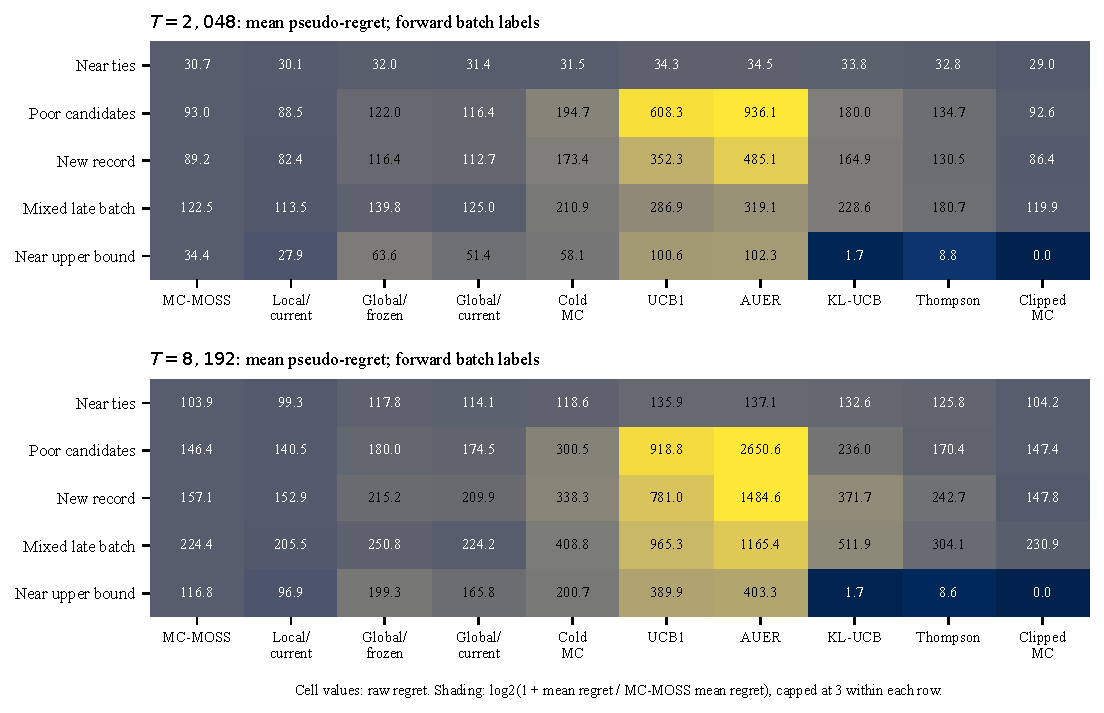
\includegraphics[width=\linewidth]{figures_v2/fig_mechanisms_baselines.pdf}
\caption{Complete forward-label mean pseudo-regrets for both horizons.
Numbers report raw regret.  Color encodes
$\log_2(1+\overline R_{\rm method}/\overline R_{\rm MC})$, capped at three
for display, within each row; it does not encode sampling uncertainty.
The tables in the released CSV files give Monte Carlo standard errors
and the reverse-label results for every cell.  The exact boundary anchor
explains the zero for the clipped rule in the last row.}
\label{fig:mechanisms-baselines-all}
\end{figure}

\begin{figure}[p]
\centering
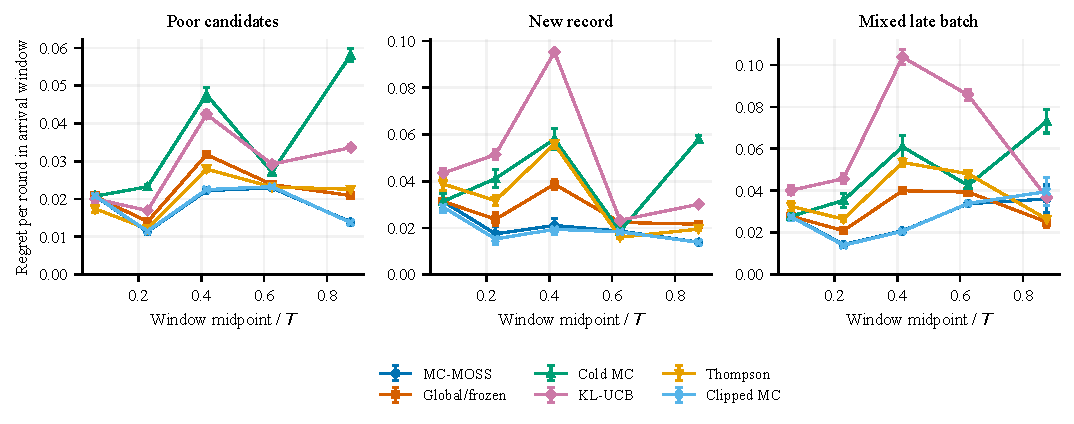
\includegraphics[width=\linewidth]{figures_v2/fig_mechanisms_windows.pdf}
\caption{Mean regret per round in the five intervals between consecutive
batch arrivals, at $T=8192$ with forward labels.  Bars are $1.96$ Monte
Carlo standard errors.  In the new-record configuration the fourth
interval begins with the arrival of the arm of mean $0.80$; in the mixed
configuration the fifth interval begins with the last heterogeneous
batch.  Window midpoints indicate the horizontal positions; connecting
segments are guides to the eye.}
\label{fig:mechanisms-windows}
\end{figure}

The software audit compared 2,316 MC-MOSS and cold-reset decisions with
the original online implementation.  It also checked 60 prefixes after
removing all future arm labels, 60 exact reruns, 800 direct evaluations of
the factorial index formulas, and 189 KL roots against an independent
Brent solver.  The largest root discrepancy was $9.37\times10^{-11}$.
Three posterior-moment checks used $10^5$ beta draws each.  These checks
validate the implementation and its information restrictions; they do
not establish regret guarantees for the experimental baselines.
